% \setchapterpreamble[u]{\margintoc}
\chapter{Models of type theory}
\labch{models}

Justifying a logic is often achieved using \emph{models}. A model consists
in giving an interpretation to all constructs of the logic we want to study,
such that its rules are still verified.
There are several ways to get models of type theory, I will present some of the
most common ones in this chapter, though my means of choice will presented in
depth in \nrefch{translations}.

\section{What is a model?}

A model of type theory is an interpretation of the concepts of a type theory
into another theory or object, both living in the same meta-theory.
\begin{figure}[hb]
  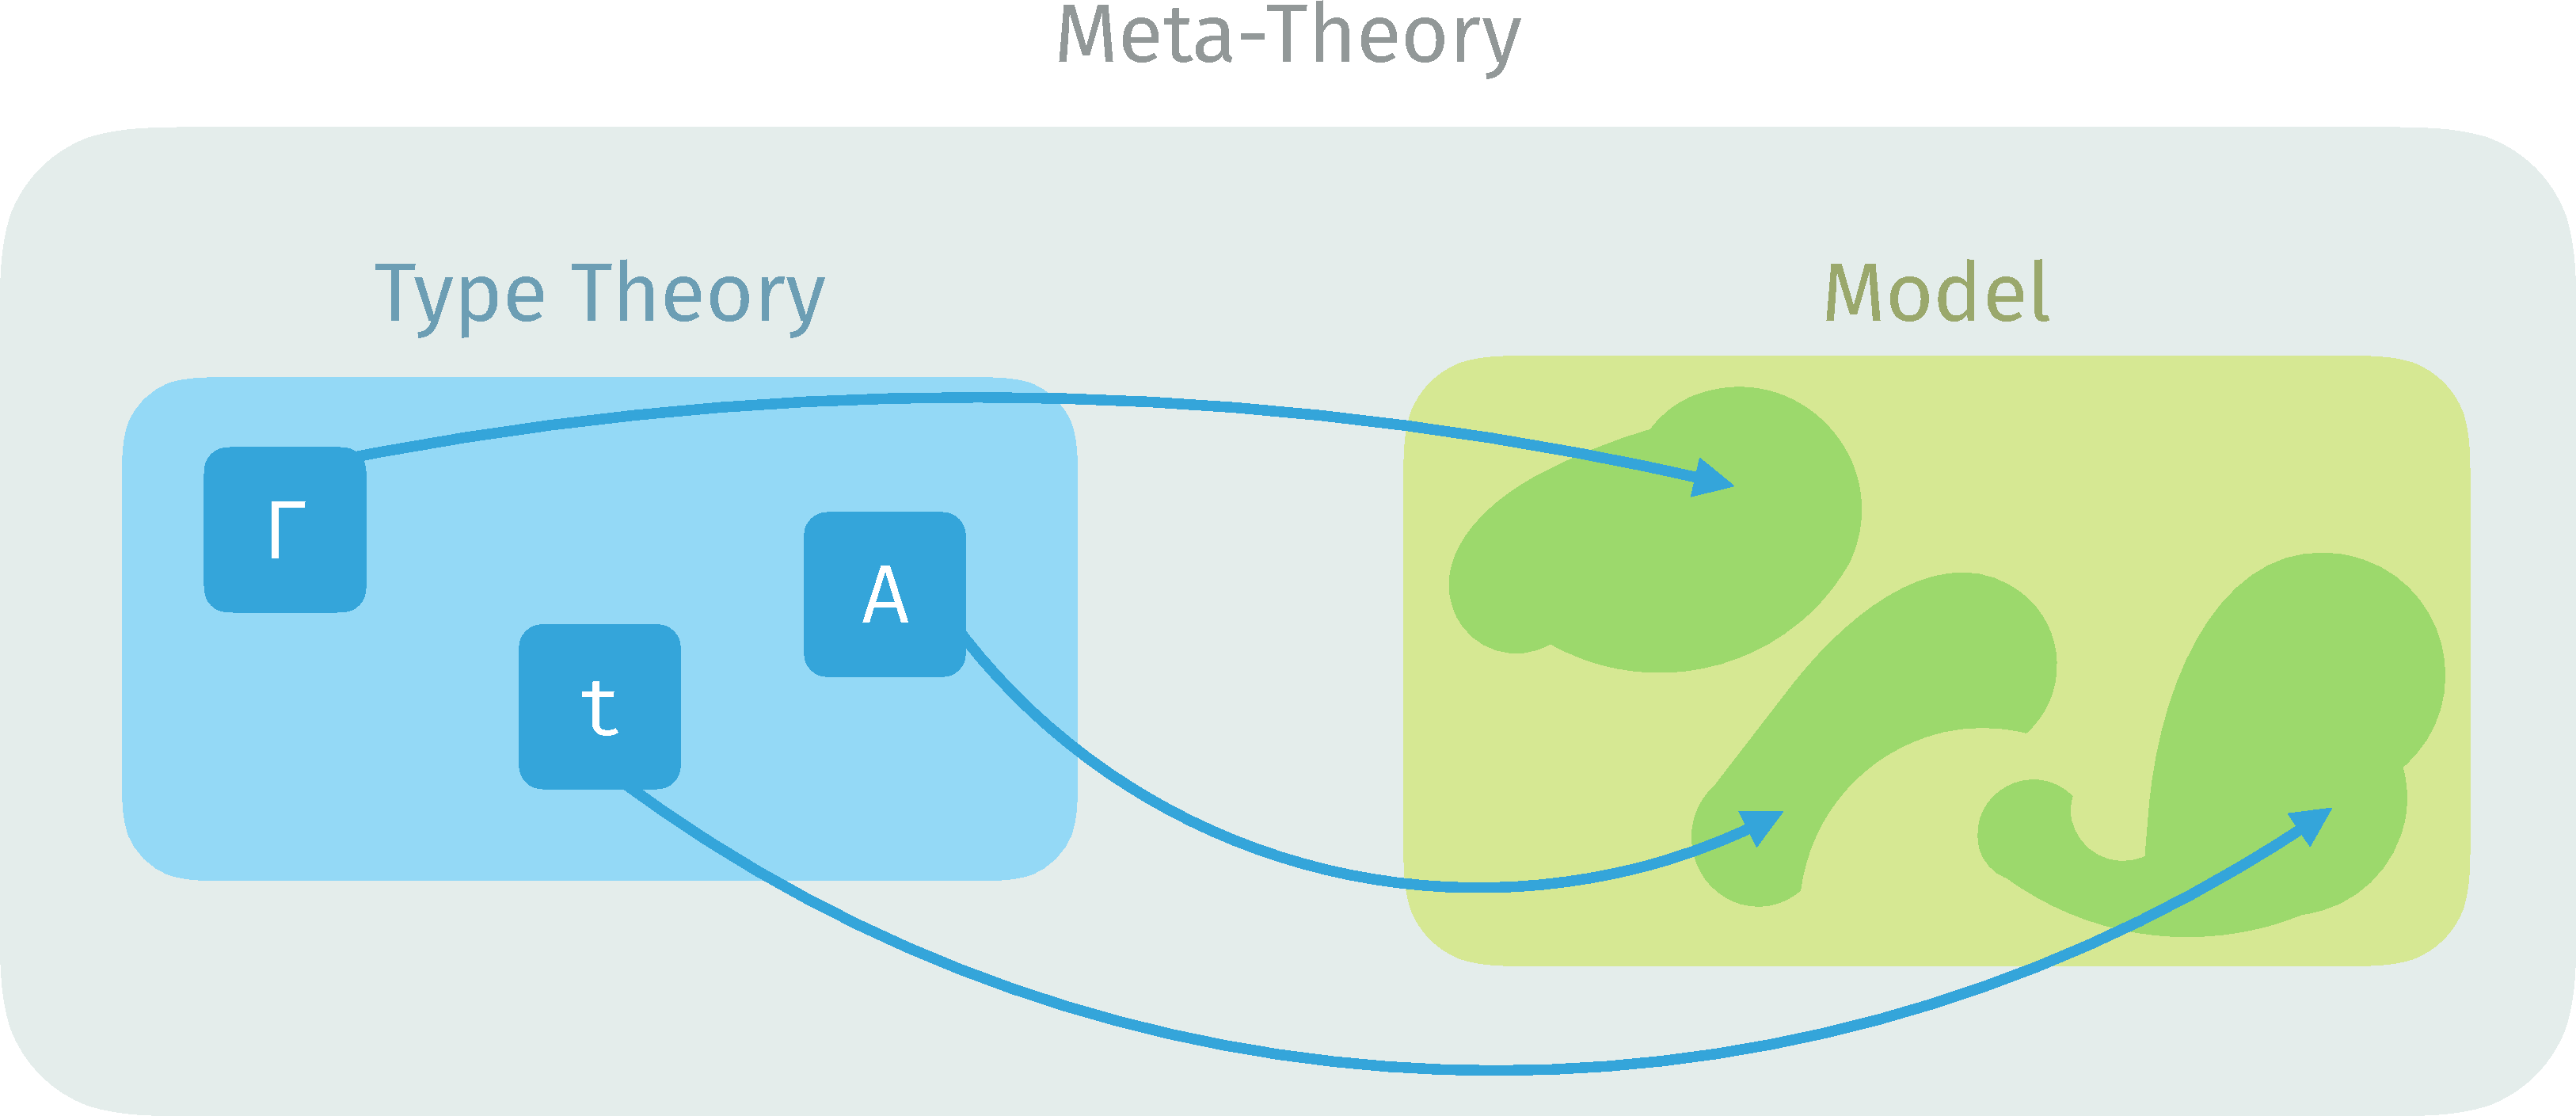
\includegraphics[width=0.9\textwidth]{model}
\end{figure}
To be more precise, a model is given by a class of objects to interpret
contexts, one for terms and one for types; but a model also provides an
interpretation to judgments in such a way that interpretation is coherent.
\todo{Make the definition clearer.}

\subsection{What can be proved using models}

\paragraph{Consistency.}

I already briefly mentioned this but the main point of models is to prove
consistency of a theory, relying on the already \emph{known} consistency of the
theory in which lives the model... At least in principle. It is however very
rare\sidenote{Impossible?} to \emph{know} that a theory is consistent, instead
we should see it as a theory we \emph{trust}, typically a theory that's widely
accepted as beeing consistent by the community of mathematicians.
This also applies to the meta-theory in which we show that the interpretation is
correct. As such it is best to keep it as simple as possible to avoid relying on
the consistency of too complicated objects.

\paragraph{Independence.}

Another interesing application of models is showing \emph{independence} of a
proposition.

\begin{definition}[Independent proposition]
  A proposition \(P\) is said to be independent from a theory \cT when neither
  \(P\) nor \(\neg P\) can be proven within \cT.
\end{definition}

A way to prove that some \(P\) is independent from \cT is to give a model of \cT
which validates \(P\) and another model which invalidates it (or validates
\(\neg P\)). Indeed if any one of \(P\) or \(\neg P\) %, let's say \(P\),
could be proven in \cT, then it would be valid in both models, leading to
at least one of them being inconsistent.

The fact that a proposition can neither be validated or invalidated in a theory
can come as surprising for some, especially in a classical mindset.
\reminder[-1.8cm]{Classical logic}{
  Classical logic is often characterised by the presence of the \acrshort{LEM}
  which consists in a proof of \(A \vee \neg A\).
}
Gödel's incompleteness theorems have to do with this.

\subsection{Gödel's incompleteness theorems}

\todo{Is it really the place? Should it even go in the proof theory chapter?}

\section{Set-theoretic models}

\section{Categorical models}

\section{Type-theoretic models}

\todo{translations, syntactical models, standard model}